\begin{figure}[ht]
    \centering
    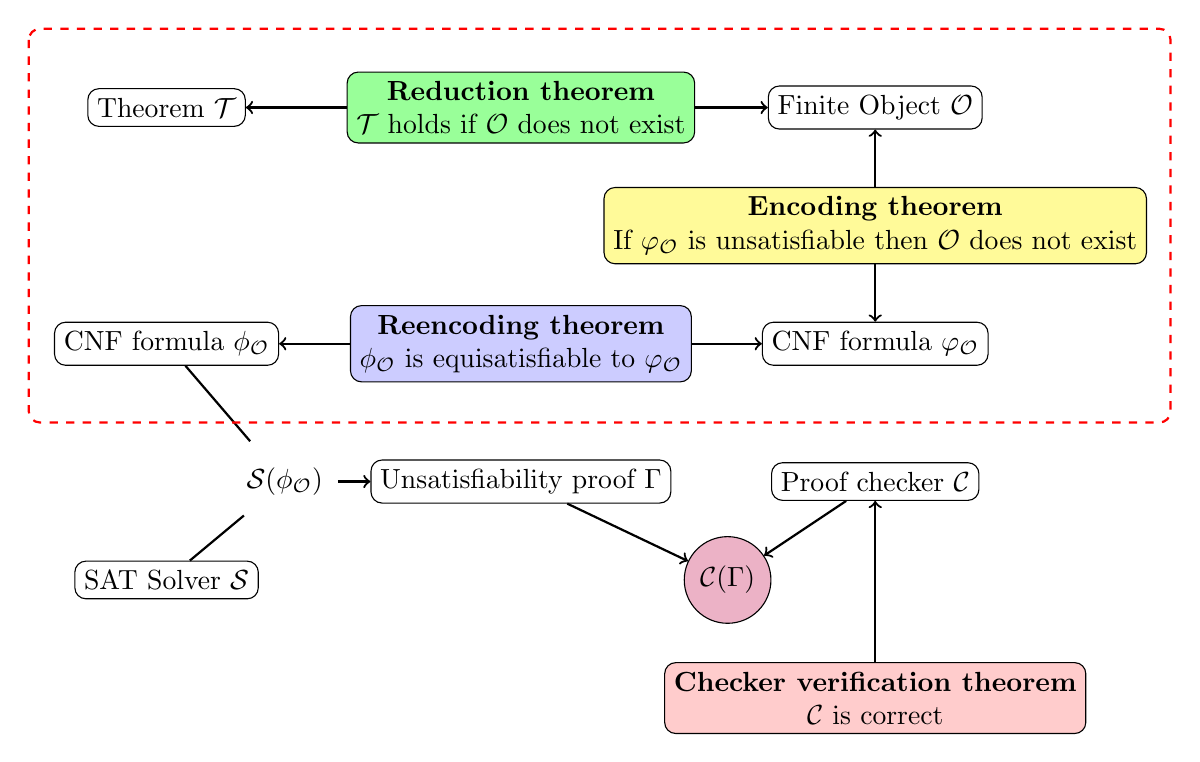
\begin{tikzpicture}
      \node[draw, rounded corners] (theorem) at (0,0) {Theorem $\mathcal{T}$};
      \node[draw, rounded corners] (object) at (9,0) { Finite Object $\mathcal{O}$};
      \node[draw, rounded corners, align=center, fill=green!40!white] (tiffo) at (4.5,0) { \textbf{Reduction theorem}\\$\mathcal{T}$ holds if $\mathcal{O}$ does not exist};
      \draw[->, thick] (tiffo) -- (theorem);
      \draw[->, thick] (tiffo) -- (object);
      \node[draw, rounded corners, align=center] (varphi) at (9, -3) {CNF formula $\varphi_{\mathcal{O}}$};
      \node[draw, rounded corners, align=center, fill=yellow!40!white] (encoding) at (9, -1.5) { \textbf{Encoding theorem}\\If $\varphi_{\mathcal{O}}$ is unsatisfiable then $\mathcal{O}$ does not exist};
      \draw[->, thick] (encoding) -- (object);
      \draw[->, thick] (encoding) -- (varphi);
      \node[draw, rounded corners] (phi) at (0, -3) {CNF formula $\phi_{\mathcal{O}}$};
      \node[draw, rounded corners, align=center, fill=blue!20!white] (equisat) at (4.5, -3) { \textbf{Reencoding theorem}\\$\phi_{\mathcal{O}}$ is equisatisfiable to $\varphi_{\mathcal{O}}$};
      \draw[->, thick] (equisat) -- (phi);
      \draw[->, thick] (equisat) -- (varphi);
      \node[draw, rounded corners] (solver) at (0, -6) {SAT Solver $\mathcal{S}$};
      \node[draw, rounded corners] (unsat-proof) at (4.5, -4.75) {Unsatisfiability proof $\Gamma$};
      \node[circle] (solverphi) at (1.5, -4.75) {$\mathcal{S}(\phi_{\mathcal{O}})$};
      \draw[-, thick] (solver) -- (solverphi);
      \draw[-, thick] (phi) -- (solverphi);
      \draw[->, thick] (solverphi) -- (unsat-proof);
      \node[draw, rounded corners] (checker) at (9, -4.75) {Proof checker $\mathcal{C}$};
      \node[circle, draw, fill=purple!30!white] (checkerphi) at (7.125, -6) {$\mathcal{C}(\Gamma)$};
      \draw[->, thick] (unsat-proof) -- (checkerphi);
      \draw[->, thick] (checker) -- (checkerphi);
      \node[draw, rounded corners, align=center, fill=red!20!white] (checkerCorrectness) at (9, -7.5) { \textbf{Checker verification theorem}\\$\mathcal{C}$ is correct};
  
      \draw[->, thick] (checkerCorrectness) -- (checker);
      \draw[red, dashed, thick, rounded corners] (-1.75,1) -- (-1.75, -4) -- (12.75, -4) -- (12.75, 1) -- cycle;
    \end{tikzpicture}
    \caption{General structure of the verification pipeline for a SAT-based theorem in the \emph{negative case}. The dashed rectangle encloses the main focus of this paper, whereas for the rest of the proof we leverage already existing tools.}\label{fig:proof-structure}
  \end{figure}